\section{The pre-registered hypotheses and decision rules}
\label{app:prereg}

The pre-registration (frozen 2026-09-23; an English translation of the binding original is in the repository with the
commands that verify its hash) fixed the grid of Section~\ref{sec:grid}, the fitting protocol of
Section~\ref{sec:measurement} and these decision rules. Before any data, three changes were made and dated in the
deviation log: the training data moved from sample-100BT to sample-10BT, which removed the $80N$ point of the 160M dense
model; the data point moved from the mean of a cooldown's last three evaluations to its final evaluation, the
three-point mean becoming a robustness variant (Table~\ref{tab:robust}); and a variant that counts $N$ without the output
head was added.

\begin{table}[h]
  \centering
  \caption{The four pre-registered hypotheses, their frozen decision rules and their verdicts.}
  \label{tab:verdicts}
  \footnotesize
  \begin{tabular}{p{0.19\linewidth}p{0.36\linewidth}p{0.36\linewidth}}
    \toprule
    Hypothesis & Decision rule for support & Verdict \\
    \midrule
    H1: truncated backpropagation lowers $\varphi$ & $\varphi_{\mathrm{trunc}} < \varphi_{\mathrm{full}}$ with
    non-overlapping 95\% bootstrap intervals, under both equal-token and equal-FLOP accounting; if only under equal
    tokens, the effect is attributed to the reallocation of FLOPs. & Not supported. Middle block 0.00 vs 0.13 (predicted
    direction, intervals overlap); whole stack 0.17 vs 0.00 (opposite direction). The equal-FLOP accounting agrees. \\
    H2: a looped middle block has a higher $\varphi$ than a looped whole stack & $\varphi_{\mathrm{mid}} >
    \varphi_{\mathrm{whole}}$ with non-overlapping intervals; raw-loss pairs of similar executed depth (middle block
    $r = 8$ vs whole stack $r = 4$; middle block $r = 4$ vs whole stack $r = 2$) are reported alongside, and a
    disagreement is reported as ``depends on the measure''. & Depends on the measure. $\varphi$ is mixed; raw losses at
    similar executed depth (36 against 32 and 20 against 16 layers) favour the middle block in 24 of 24 comparisons, by
    0.03--0.19 nats, less at larger sizes. \\
    H3: $\varphi$ saturates in $r$ & The geometric form has the lower extrapolation error in both directions (10M--40M
    predicting 80M; 20M--80M predicting 10M) and an information-criterion difference above 10. & Not supported. The
    geometric form predicts 80M from 10M--40M better (0.0085 vs 0.0096 rmse) and 10M from 20M--80M slightly worse
    (0.0203 vs 0.0200); the data do not separate the two forms. \\
    H4: the compute-optimal $r$ & Under matched training FLOPs the optimal $r \leq 2$, under matched deployment FLOPs
    larger; computed from the fitted law, without a test. & First half holds trivially (the dense model, $r = 1$, is
    optimal under training compute); second half not supported (it is optimal under deployment compute too). \\
    \bottomrule
  \end{tabular}
\end{table}

A factor effect counts only if it exceeds both the bootstrap half-width and the spread of $\varphi$ fitted separately
to the three seeds at 20M and 40M. The information criterion of H3 turned out to be computable only as a proxy from the
Huber loss, which is not a likelihood; it is not used as evidence (Appendix~\ref{app:deviations}). Two rules were added
during the grid, after the first spikes (2026-09-26) and after the collapse (2026-09-30), each before the results it
governs existed, and are dated in the deviation log: spikes are reported per run with a robustness fit without the runs that have them, and a cooldown result enters no fit
if its branch starts after a collapse or ends more than 1.0 nats above the lowest trunk loss before it (four results of
two runs: three of a 40M whole stack looped 8 times with truncation, seed 43, which collapsed, and the $10N$ result of a
40M whole stack looped 8 times with full backpropagation, seed 44, after a severe spike).

\section{Training details}
\label{app:training}

Table~\ref{tab:sizes} lists the sizes and Table~\ref{tab:supp} the supplementary experiments.

\begin{table}[h]
  \centering
  \caption{Model sizes and training settings on text. Size names give the approximate non-embedding parameters; $N$
  also counts the output head \citep{porian2024resolving}, which is large at small widths with a 16k vocabulary. The
  looped models of a size have the same unique layers plus a $2w^2$ injection map (under 2\% of $N$). The learning rate is that of the embedding and output layers, frozen after a
  33-run sweep; the hidden layers use $1.22$ times it. Warm-up is $2N$ tokens.}
  \label{tab:sizes}
  \small
  \begin{tabular}{lrrrrrl}
    \toprule
    Size & Width $w$ & Heads & $N$ & Tokens per step & Learning rate & Seeds (dense / looped) \\
    \midrule
    10M  & 320  & 5  & 15.4M  & 81,920  & $2.19\times10^{-3}$ & 3 / 3 \\
    20M  & 448  & 7  & 26.8M  & 131,072 & $1.53\times10^{-3}$ & 3 / 3 \\
    40M  & 640  & 10 & 50.1M  & 204,800 & $1.83\times10^{-3}$ & 3 / 3 \\
    80M  & 896  & 14 & 92.7M  & 327,680 & $2.03\times10^{-3}$ & 1 / 1 \\
    160M & 1280 & 20 & 179.6M & 524,288 & $1.56\times10^{-3}$ & 2 / 2 (middle block, $r=4$) \\
    \bottomrule
  \end{tabular}
\end{table}

\begin{table}[h]
  \centering
  \caption{The ten supplementary experiments, each run under a plan frozen before its runs (the S8 plan was written after
  the frozen stopping rule's results on the same checkpoints were known).}
  \label{tab:supp}
  \footnotesize
  \begin{tabular}{llll}
    \toprule
    & Plan frozen & What it adds & Where \\
    \midrule
    S1  & 2026-10-13 & Learning rates re-tuned for the dense model and a middle block looped 4 times & \S\ref{sec:multiplier}, App.~\ref{app:lr} \\
    S2  & 2026-10-13 & Learning rate and learning of the chain task, three seeds & \S\ref{sec:lrsynthetic} \\
    S3  & 2026-10-13 & Inference cost & \S\ref{sec:cost}, App.~\ref{app:cost} \\
    S4  & 2026-10-15 & Dense models continued to $640N$ (10M) and $320N$ (20M) & \S\ref{sec:equalcompute}, App.~\ref{app:lr} \\
    S5  & 2026-10-15 & Chain of thought and pause tokens on the chain task & \S\ref{sec:inrange}, \S\ref{sec:extension} \\
    S6  & 2026-10-15 & KV cache shared across loops after training & \S\ref{sec:cost}, App.~\ref{app:cost} \\
    S7  & 2026-10-15 & Data order & \S\ref{sec:mechanism}, App.~\ref{app:fits} \\
    S8  & 2026-10-15 & Answer-free stopping rules & \S\ref{sec:stopping}, App.~\ref{app:synthetic} \\
    S9  & 2026-10-15 & Loops = steps with 0--4 random extra loops & \S\ref{sec:stopping} \\
    S10 & 2026-10-27 & Dense models with 18 layers and the looped model's parameters & \S\ref{sec:depth}, App.~\ref{app:s10} \\
    \bottomrule
  \end{tabular}
\end{table}

\paragraph{Data.} The three further validation sets of 20M tokens each come from a 6B-token sample of SlimPajama, from
FineMath (finemath-4plus) and from GitHub code (github-code-clean,
\url{https://huggingface.co/datasets/codeparrot/github-code-clean}).

\paragraph{Extensions.} The extensions continue the 10M middle blocks looped 4 and 8 times (two seeds) to $80N$ and
$160N$, a 10M whole stack looped 4 times and a truncated one looped 8 times (one seed) to the same budgets, the 10M dense
model to $160N$ and the 20M middle blocks looped 4 and 8 times (two seeds) to $80N$.

\paragraph{Learning rates.} A sweep of 33 runs at $10N$ (30 dense runs at five rates per width, a $\beta_2 = 0.99$ group
at 20M, and three looped runs at 80M) fixed the rate per width (Table~\ref{tab:sizes}); the minima of all five widths
lie inside the swept range, and $\beta_2 = 0.95$ beat 0.99 by 0.008 nats. The hidden layers use
$\eta_0 (8/12)^{-1/2} \approx 1.22\,\eta_0$. A check for looped cells, whose decision rule was written before its runs on 2026-09-25, two days after the
pre-registration (20M, ten cells at 0.5, 0.71 and 1
times the dense rate, $10N$) found no better rate by the rule fixed in advance (pooled best multiple 0.97, threshold
0.84), so all looped language models use the dense rates. Nine of the ten cells were best at 1$\times$, the top
of that range, so higher rates were not excluded. The residual scaling of Section~\ref{sec:models} is meant to keep the
best rate independent of $r$: we found no downward shift of the best rate in this check, but at 10M with longer training
the looped model preferred lower rates (Section~\ref{sec:multiplier}).

\paragraph{FLOP accounting.} Training FLOPs count two FLOPs per multiply-add over every executed layer, the attention
terms and the output head, plus a backward pass of twice the forward cost for every layer that receives gradients; with
truncated backpropagation the backward pass covers the prelude, the coda, the output head and the last $r/2$ loops.

\paragraph{The grid at equal parameters.} Table~\ref{tab:gaps} gives the looped minus dense loss per cell and size,
averaged over the three budgets.

\begin{table}[h]
  \centering
  \caption{Looped minus dense loss at equal parameters and tokens, mean over the budgets $10N$, $20N$ and $40N$ and over
  seeds (negative: looped better). $^{*}$Includes a seed with a severe loss spike; without it, $-0.029$.}
  \label{tab:gaps}
  \small
  \begin{tabular}{lcccc}
    \toprule
    Cell & 10M & 20M & 40M & 80M \\
    \midrule
    Middle block, $r=2$ & $+0.068$ & $+0.025$ & $-0.010$ & $-0.015$ \\
    Middle block, $r=4$ & $+0.055$ & $+0.002$ & $-0.030$ & $-0.039$ \\
    Middle block, $r=4$, truncated & $+0.079$ & $+0.031$ & $+0.006$ & $+0.009$ \\
    Middle block, $r=8$ & $+0.031$ & $-0.003$ & $-0.033$ & $-0.033$ \\
    Middle block, $r=8$, truncated & $+0.039$ & $+0.001$ & $-0.022$ & $-0.018$ \\
    Whole stack, $r=2$ & $+0.172$ & $+0.079$ & $+0.021$ & $+0.003$ \\
    Whole stack, $r=4$ & $+0.150$ & $+0.085$ & $+0.047$ & $+0.025$ \\
    Whole stack, $r=4$, truncated & $+0.044$ & $+0.003$ & $-0.014$ & $+0.017$ \\
    Whole stack, $r=8$ & $-0.074$ & $-0.055$ & $+0.213^{*}$ & $-0.003$ \\
    Whole stack, $r=8$, truncated & $-0.053$ & $-0.041$ & $-0.042$ & $-0.020$ \\
    \bottomrule
  \end{tabular}
\end{table}

\paragraph{Two observations from the grid.} Truncated backpropagation, predicted to hurt, helped whole-stack loops with
four loops at every size (Table~\ref{tab:gaps}): at 20M a whole stack looped 4 times reached 3.646 with truncation and
3.783 with full backpropagation at $10N$ (three-seed means); with eight loops it was slightly worse at 10M--20M. At 10M
the only looped cells better than the dense model on average over the three budgets were whole-stack loops with
$r = 8$. Truncation and whole-stack loops also brought instability: 30 of the 111 runs had at least one loss spike, 25
with truncated backpropagation (16 of these whole-stack loops) and five whole-stack loops with $r = 8$ and full
backpropagation; one run collapsed. In an exploratory follow-up, a 10M whole stack looped 4 times with truncation,
trained at half the learning rate in three seeds, had no spike at all (4, 1 and 10 at the original rate); it was worse
by 0.044 nats at $10N$ and better by 0.064 at $40N$, which cannot be credited to the missing spikes alone, since longer
budgets also favour a lower constant rate.

\section{Fits and robustness}
\label{app:fits}

The fits use a Huber loss in log space ($\delta = 10^{-3}$), 500 random starts and 1000 block-bootstrap resamples. The
primary ruler, fitted to 54 dense results, is $E = 0.050$ (at the lower bound of the fit), $A = 6.98$,
$\alpha = 0.054$, $B = 1065$, $\beta = 0.370$; the joint fit over all 352 results gives $E = 1.94$, $A = 61.7$,
$\alpha = 0.267$, $B = 197$, $\beta = 0.266$. Under the constant-$\varphi$ model, setting every $\varphi$ to 0 raises the
Huber loss only from 0.00352 to 0.00379, and setting it to 1 raises it to 0.0142. Table~\ref{tab:robust} gives the
primary $\varphi$ under the robustness variants of the pre-registration and of the deviation log, each fixed before the
results it governs. Fitted separately to each seed, $\varphi$ varies by
0.10--0.21 per cell at 20M and 0.00--0.11 at 40M; the factor effects of Table~\ref{tab:prereg} (0.13--0.17) do not exceed
the 20M spread.

\begin{table}[h]
  \centering
  \caption{$\varphi$ (primary fit) under robustness variants, in the order middle block full / middle block truncated /
  whole stack full / whole stack truncated.}
  \label{tab:robust}
  \small
  \begin{tabular}{ll}
    \toprule
    Variant & $\varphi$ \\
    \midrule
    Primary analysis & 0.13 / 0.00 / 0.00 / 0.17 \\
    Without the 30 runs with loss spikes & 0.13 / 0.11 / 0.00 / 0.22 \\
    Mean of the last three evaluations (the pre-registered data point) & 0.14 / 0.00 / 0.00 / 0.17 \\
    Second validation set (SlimPajama) & 0.31 / 0.18 / 0.02 / 0.30 \\
    Without $r = 8$ & 0.07 / 0.00 / 0.00 / 0.07 \\
    Half the budget & 0.08 / 0.00 / 0.00 / 0.15 \\
    $N$ without the output head & 0.07 / 0.00 / 0.00 / 0.14 \\
    Equal-FLOP accounting & 0.13 / 0.08 / 0.00 / 0.16 \\
    \bottomrule
  \end{tabular}
\end{table}

For H3, the pre-registered extrapolation (10M--40M to 80M and 20M--80M to 10M, with the dense-only 160M size in neither
training set) gives a root-mean-square error of 0.0096 and 0.0200 for $r^{\varphi}$ and 0.0085 and 0.0203 for the
geometric form. Five of the seven robustness variants show the same split; without $r = 8$ the split is reversed, and
on the second validation set $r^{\varphi}$ is better in both directions. For H4, the fitted law makes the dense model
optimal at every training budget from $10^{17}$ to $10^{20}$ FLOPs, with the smallest available $r$ the best looped
choice, 0.00--0.17 nats behind; under deployment compute the dense model is optimal as well, with either set of ruler
parameters.

\paragraph{Loop-by-loop probes of the language models.} The state after each loop $k$ is read in three ways: with the
model's own output layers (the logit lens of \citealp{nostalgebraist2020logit}, which here is the same as running the
model with $k$ loops), with a learned linear $w\times w$ map in front of the output layers (in the spirit of the tuned
lens of \citealp{belrose2023tuned}, but trained on the next token rather than distilled from the model's own output),
and with a learned linear head; the maps are trained on 10M unseen training tokens and evaluated on 2M tokens of the
main validation set.

\paragraph{The multiplier plane.} A least-squares plane in $\log_2 M$ over the middle block looped 4 times gives a
factor of 1.21 per doubling of model size and 1.14 per doubling of tokens per parameter (1.16 with 8 loops), with
classical 95\% intervals, which include the plane's misfit, of 1.13--1.30 and 1.05--1.24; by these intervals the product
term is indistinguishable from zero. On the plane the loop breaks even ($M = 1$) at about $N = 35$M with 20 tokens per
parameter and at about $N = 12$M, below the smallest model, with 80; the measured points agree at 80 (1.04 for the 10M
model, 1.05 on the plane) but reach $M = 1$ earlier at 20 (the 20M model is at 0.99, the plane at 0.93). At 10M with 10
tokens per parameter the two dense models measured at that number of tokens are out of order (the 20M one, at 5.7
tokens per parameter, is worse than the 10M one), so $\Nstar$ cannot be extrapolated either.

\paragraph{Published multipliers.}\label{app:published} Published equal-parameter results mostly restate to a similar range in comparable settings, and to higher values at
larger sizes or with far more tokens per parameter. Where a paper reports a non-looped ladder, we interpolate it in the
same way. Parcae's models, trained with a loop count sampled around a mean of 8 and backpropagated through 4 of them,
and run with 8, are worth 1.31--1.46 dense parameters per parameter at 140M--770M \citep{prairie2026parcae}, against a
ladder trained on the same tokens per parameter, which understates the value. Ouro's models looped 4 times are worth
1.23 and 1.36 at 134M and 374M (about 150 and 50 tokens per parameter) and more than 1.75 at 778M, beyond its largest
non-looped model, but less than their parameters at 53M despite about 380 tokens per parameter, measured by mean
benchmark accuracy read off a plot (\citealp[App.~D.1]{zhu2025scaling}). The two 12-layer looped models of \citet{saunshi2025reasoning}, about 0.5B
parameters looped 2 and 4 times, are worth 1.26 and 1.36, and their shallower blocks looped 3, 4 and 6 times
1.47--1.95, at about 750--1500 tokens per parameter. The law of \citet{schwethelm2026how} ($\varphi = 0.46$, 95\% interval 0.41--0.53) implies 1.25, 1.45 and 1.56
for 2, 4 and 8 loops in their iso-depth layouts. These studies differ from ours in size, data and recipe, so the
agreement is a consistency check, not a pooled estimate. They barely sample models below 40M trained on 20 or fewer
tokens per parameter, where we find a model with a looped middle block worth at most about as many dense
parameters as it has. That the value rises with tokens per
parameter at equal parameters is a dependence that effective-parameter laws whose loop gain depends on the loop
count (and, for mixtures of experts, on the sparsity) but not on the training tokens
\citep{schwethelm2026how,chen2026moe} do not capture; it agrees with the recommendation of \citet{prairie2026parcae} to
increase looping and data in tandem, and with the finding of \citet{chen2026growth} that with repeated data the best
loop count grows with compute.

\paragraph{Where the gain lands, and what the seeds measure.} Per token, the gain on web text is a small, broad shift:
about half of the tokens improve, and the gain is not concentrated on hard tokens beyond what two dense seeds differ by
\lbl{(exploratory)}. On math and code text the gain is larger, on average about 3 and 7 times the gain on the main set,
but the seed-to-seed spread on those sets is 10--100 times larger as well. Supplementary experiment S7
\lbl{(pre-specified)} showed that the code set is even more sensitive to the data order, which our seeds share, than to
the initialisation (the math set is not): at 20M, training the same initialisation on three disjoint parts of the data
stream moves the main-set loss by only 0.003--0.011 nats, 0.1--0.5 times the spread between initialisation seeds (the plan
had predicted one to three times), but moves the code-set loss by 0.21--0.69 nats, up to 7 times that spread, and changes
the sign of the looped-minus-dense gap there. Of the plan's four predictions only this one, a code-set spread above 0.1,
held: on the main set the data-order spread was smaller than predicted relative to the initialisation spread (and, for
the dense model, below the predicted 0.005--0.02 nats), and the looped-minus-dense gap did not vary less than the losses. Both the initialisation and the documents a run happens to see move its out-of-distribution loss strongly at this
size, so we draw no conclusions from differences on those sets.

\section{Learning rates (S1) and equal compute at the largest budgets (S4)}
\label{app:lr}

S1 re-tuned the dense model and the middle block looped 4 times at 10M, 20M and 40M: 0.5 to 1.41 times the dense rate,
plus 0.35 times where the best rate lay at the lowest one tried, at $10N$--$40N$ (at 10M also $80N$ and $160N$), with one
seed (two at 20M). Table~\ref{tab:s1} gives the gap between the middle block looped 4 times and the dense model at the
shared rate
($\Delta_1$) and with each model at its best rate ($\Delta^{\star}$), and $h = \Delta_1 - \Delta^{\star}$, the bias of
the shared rate against the looped model. The pre-specified readings: the trend with size holds (at $40N$ the
improvement from 10M to 40M is 0.050 against 0.065 at the shared rate, above the threshold of half of it), the trend
with data holds and grows (10M from $10N$ to $160N$: 0.141 against 0.119), the equal-compute verdict was unchanged
at the time (its 10M comparison at $160N$, extrapolated then, was later measured in S4: $-0.011$, a looped advantage, and
$+0.005$ with a second seed; Section~\ref{sec:equalcompute}), and
the bias exceeds the 0.01 tolerance at 10M only.

\begin{table}[h]
  \centering
  \caption{S1: looped (middle block, $r = 4$) minus dense loss at the shared rate and at each model's best rate (seed 42;
  20M: mean of seeds 42 and 43). $^{\dagger}$The lowest rate tested.}
  \label{tab:s1}
  \small
  \begin{tabular}{lcccc}
    \toprule
    Size, budget & $\Delta_1$, shared rate & $\Delta^{\star}$, best rates & $h$ & Best rate, dense / looped \\
    \midrule
    10M, $10N$  & $+0.082$ & $+0.082$ & $+0.000$ & 1 / 0.71 \\
    10M, $20N$  & $+0.044$ & $+0.026$ & $+0.018$ & 1 / 0.5 \\
    10M, $40N$  & $+0.015$ & $-0.005$ & $+0.020$ & 1 / 0.5 \\
    10M, $80N$  & $-0.010$ & $-0.035$ & $+0.024$ & 1 / 0.35$^{\dagger}$ \\
    10M, $160N$ & $-0.037$ & $-0.059$ & $+0.022$ & 1 / 0.35$^{\dagger}$ \\
    20M, $10N$  & $+0.028$ & $+0.028$ & $0.000$ & 1 / 1 \\
    20M, $20N$  & $-0.005$ & $-0.005$ & $0.000$ & 1 / 1 \\
    20M, $40N$  & $-0.031$ & $-0.031$ & $0.000$ & 1 / 1 \\
    40M, $10N$  & $-0.008$ & $-0.008$ & $0.000$ & 1 / 1 \\
    40M, $20N$  & $-0.032$ & $-0.036$ & $+0.004$ & 1 / 0.71 \\
    40M, $40N$  & $-0.050$ & $-0.055$ & $+0.005$ & 0.71 / 0.71 \\
    \bottomrule
  \end{tabular}
\end{table}

On the trunk checkpoints at $32N$, the range of the main-set loss over 4--16 inference loops is 0.30, 0.36, 1.02, 3.39
and 4.10 nats at 0.35, 0.5, 0.71, 1 and 1.41 times the dense rate at 10M, 0.53--3.42 at 20M and 0.77--4.81 at 40M
(0.5 to 1.41 times): lower rates make the iteration closer to convergent, but at every rate the better of 8 and 16 loops
is worse than the 4 loops of training, by 0.07--3.0 nats.

\paragraph{Extrapolated equal-compute comparisons.} Two extrapolations bracket a dense loss beyond the measured curve:
in a backtest that drops the last budgets of every measured dense curve, extending the last segment predicts a dense
loss 0.023--0.036 nats too low one doubling out (it flatters the dense model), and a power law fitted to the whole curve
one 0.006--0.027 too high (it flatters looping). After S4, 62 equal-compute comparisons still need an extrapolated dense
loss: 43 at 40M--160M, and 19 at 10M--20M, almost all for the third seed, whose dense curve ends at $80N$. At 160M and
$40N$ the bracket reaches from $+0.004$ to $+0.043$.

\paragraph{Equal compute at the largest budgets (S4).} Table~\ref{tab:equalcompute} gives the equal-compute comparisons at the
largest looped budgets. The S4 plan had predicted gaps between $-0.01$ and $+0.04$, the dense model ahead in most and none
below $-0.02$; the last two held, but four of the nine measured top-budget gaps exceeded $+0.04$ (up to $+0.054$).

\begin{table}[h]
  \centering
  \caption{The equal-compute comparisons at the largest looped budgets (S4; looped minus dense loss on the main
  validation set, means over two seeds; negative: looped better). At equal compute the dense model is trained on 2.2--3.8
  times the tokens.}
  \label{tab:equalcompute}
  \footnotesize
  \begin{tabular}{lccc}
    \toprule
    & Training FLOPs & \multicolumn{2}{c}{Looped $-$ dense loss} \\
    \cmidrule(lr){3-4}
    Looped cell (size, tokens per parameter) & vs dense & equal parameters and tokens & equal compute \\
    \midrule
    Middle block, $r=4$ (10M, $160N$) & 2.2$\times$ & $-0.033$ & $+0.016$ \\
    Middle block, $r=8$ (10M, $160N$) & 3.7$\times$ & $-0.051$ & $+0.034$ \\
    Middle block, $r=4$ (20M, $80N$)  & 2.2$\times$ & $-0.051$ & $+0.022$ \\
    Middle block, $r=8$ (20M, $80N$)  & 3.8$\times$ & $-0.064$ & $+0.052$ \\
    \midrule
    Middle block, $r=4$, 0.35$\times$ rate (10M, $160N$) & 2.2$\times$ & --- & $-0.011$, $+0.005$ (seeds) \\
    \bottomrule
  \end{tabular}
\end{table}

\section{Depth or sharing (S10)}
\label{app:s10}

The plan was frozen on 2026-10-27, before any of its runs. Dense models with 18 layers and the looped model's number of
parameters (Table~\ref{tab:s10}) were trained with the recipe of the grid's runs of the same size: the same data in the
same order, batch, warm-up and optimiser settings, one constant-rate trunk with cooldown branches ending at $10N$, $20N$
and $40N$ of that size (in tokens identical to the looped runs), the same evaluation sets, and seeds 42, 43 and 44. The
embedding and output layers use the frozen rate of their width ($2.19\times10^{-3}$ at width 320, $1.53\times10^{-3}$ at
448) and the hidden layers $(18/12)^{-1/2}$ times it, as the code does for any depth; seed 42 was also trained at 0.71
and 1.41 times that rate. Training FLOPs per token are 205M (dense, 8 layers), 456M (looped) and 239M (dense, 18 layers)
at 20M, and 364M, 835M and 406M at 40M. None of the ten runs had a loss spike.

\begin{table}[h]
  \centering
  \caption{S10: dense models with 18 layers ($18 \times 320$, $N = 28.1$M; $18 \times 448$, $N = 51.2$M) against the
  middle block looped 4 times (8 unique layers, 20 executed; $N = 27.2$M and 51.0M), at the rule's learning rate. Losses
  and gaps are means over three seeds (the gap per seed in parentheses; positive: looped better); $M$ is read off the
  8-layer dense ruler; 95\% intervals from resampling seeds. At 20M the plan reports the results descriptively:
  $M_{\mathrm{loop}}$ is near 1 at $10N$ and $20N$, and $R$ is unstable (0.58, 10.1 and $-0.40$).}
  \label{tab:s10}
  \footnotesize
  \setlength{\tabcolsep}{2.6pt}
  \begin{tabular}{lcccccc}
    \toprule
    Size, budget & Dense, 18 layers & Looped & Gap (seeds) & $M_{\mathrm{deep}}$ & $M_{\mathrm{loop}}$ & $R$ \\
    \midrule
    20M, $10N$ & 3.654 & 3.671 & $-0.017$ ($-0.010$, $-0.016$, $-0.026$) & 0.84 [0.76, 0.98] & 0.74 [0.67, 0.83] & --- \\
    20M, $20N$ & 3.465 & 3.456 & $+0.008$ ($+0.017$, $+0.013$, $-0.005$) & 0.92 [0.85, 1.01] & 0.99 [0.92, 1.11] & --- \\
    20M, $40N$ & 3.335 & 3.307 & $+0.028$ ($+0.037$, $+0.033$, $+0.015$) & 0.94 [0.89, 1.00] & 1.16 [1.09, 1.25] & --- \\
    40M, $10N$ & 3.397 & 3.394 & $+0.003$ ($+0.004$, $+0.004$, $-0.001$) & 1.10 [1.04, 1.14] & 1.15 [1.08, 1.20] & 0.67 [0.43, 1.03] \\
    40M, $20N$ & 3.232 & 3.217 & $+0.015$ ($+0.017$, $+0.018$, $+0.010$) & 1.11 [1.09, 1.13] & 1.26 [1.21, 1.29] & 0.46 [0.38, 0.55] \\
    40M, $40N$ & 3.119 & 3.090 & $+0.029$ ($+0.030$, $+0.032$, $+0.026$) & 1.11 [1.10, 1.12] & 1.34 [1.31, 1.36] & 0.36 [0.32, 0.41] \\
    \bottomrule
  \end{tabular}
\end{table}

\paragraph{Readings fixed in advance.} The primary reading is $R$ at 40M averaged over the three budgets: at least 0.75
reads as ``most of the advantage is a depth effect'', 0.25--0.75 as ``partly depth, partly sharing'' and below 0.25 as
``looping buys more than depth''. It is 0.50 (95\% interval 0.41--0.62). The plan would also have reported the two
models as on par at 40M had the gap been within 0.01 nats at all three budgets; it is not ($+0.015$ and $+0.029$ at $20N$
and $40N$).

\paragraph{Learning rate.} Seed 42 at 0.71, 1 and 1.41 times the rule's rate: at 40M 3.421, 3.396 and 3.382 at $10N$,
3.246, 3.231 and 3.225 at $20N$, and 3.126, 3.118 and 3.117 at $40N$; at 20M the rule's rate was the best at every
budget. Because 1.41 times the rate beat the rule's rate by more than 0.01 nats at 40M and $10N$ (by 0.014), the plan
asks for the readings also at the best rate tried, as in S1, the primary reading staying at the rule's rate. With each
model at its best tested rate (seed 42; the looped model's best rates, from S1, are 1, 0.71 and 0.71 times the dense
rate at $10N$, $20N$ and $40N$; both read off the 8-layer dense runs at their frozen rates, seed means, with
\texttt{fit/supp3\_best\_lr.py}), the gap is $-0.010$, $+0.015$ and $+0.036$, $M_{\mathrm{deep}}$ 1.37, 1.17 and 1.12,
$M_{\mathrm{loop}}$ 1.18, 1.33 and 1.41, and $R$ 1.91, 0.56 and 0.34 (mean 0.94; for seed 42 at the rule's rate 0.58,
0.45 and 0.37, mean 0.47). The mean at the best rates falls in the band the plan reads as ``most of the advantage is a depth effect''; it is
carried by $10N$, where $\log M_{\mathrm{loop}}$ is smallest, and the primary reading stays at the rule's rate.
The analysis script written before the results flagged this case but did not compute these readings; they come from a
script written afterwards that implements the rule of the plan.

\paragraph{Predictions.} The plan predicted $R$ at 40M between 0.25 and 0.75 (held: 0.50); the 18-layer dense model
better than the 8-layer one of the same size by 0.01--0.03 nats at 40M (0.007, 0.016 and 0.020 at $10N$, $20N$ and $40N$:
held at two of the three budgets; at 20M it is worse by 0.014, 0.008 and 0.003); and the rule's rate within 0.01 nats of
the best of the three (held at five of the six budgets).

\paragraph{Equal compute \lbl{(exploratory)}.} Read as in Section~\ref{sec:equalcompute}, without extrapolation: the
looped model is behind the 18-layer dense model of equal training compute by 0.166 nats at 40M and $10N$ (compute ratio
2.05) and by 0.193 and 0.112 at 20M and $10N$ and $20N$ (ratio 1.91).

\section{Deployment measurements}
\label{app:cost}

Inference was timed on one RTX 4090 (all other GPUs idle) in bf16, with the decoding step in a CUDA graph, one KV-cache
slot per executed layer, random weights, a 512-token prompt and 512 generated tokens, at batch 1 and 32. Table~\ref{tab:s3} gives the ratios at
equal loss for all middle-block and whole-stack cells, against the dense model that reaches the same loss at $40N$
(interpolated between dense sizes).

\begin{table}[h]
  \centering
  \caption{S3: looped over dense, at equal loss. $^{*}$160M lies beyond the largest dense model (extrapolated).}
  \label{tab:s3}
  \footnotesize
  \setlength{\tabcolsep}{4pt}
  \begin{tabular}{llccccc}
    \toprule
    & & Weight & KV cache & Decoding time & \multicolumn{2}{c}{Peak memory} \\
    \cmidrule(lr){6-7}
    Cell & Sizes & memory & per token & batch 1 & batch 1 & batch 32 \\
    \midrule
    Middle block, $r=2$ & 20M--80M  & 0.93--1.03 & 1.43--1.51 & 1.45--1.49 & 0.99--1.15 & 1.21--1.24 \\
    Middle block, $r=4$ & 20M--160M & 0.81$^{*}$--0.96 & 2.20--2.41 & 2.37--2.47 & 0.98$^{*}$--1.20 & 1.57--1.58 \\
    Middle block, $r=8$ & 20M--80M  & 0.83--0.92 & 4.01--4.23 & 4.27--4.56 & 1.08--1.34 & 2.29--2.40 \\
    Whole stack, $r=4$  & 20M--80M  & 1.03--1.11 & 4.02--4.27 & 4.00--4.11 & 1.18--1.84 & 2.32--2.41 \\
    Whole stack, $r=8$  & 20M--80M  & 0.81--0.85 & 6.96--7.23 & 7.57--7.91 & 1.27--1.50 & 3.38--3.91 \\
    \bottomrule
  \end{tabular}
\end{table}

For KV sharing (S6), the first 262{,}144 tokens of the main validation set were decoded token by token in 256 windows of
1024, with one cache slot per executed layer (whose loss equals that of the ordinary forward pass to four decimals) and
with one slot per unique layer, written at a position's last loop and read by every later loop. The models are the 20M
trunk checkpoints at $32N$ (seed 42); Figure~\ref{fig:cost}b gives the loss differences, and the random-loop model run
with 16 loops instead of 8 also shares at no cost.

At batch 1 the larger KV cache cancels the saving in weights: the looped model needs 1--2\% less peak memory at
80M--160M and more at 20M--40M (up to 1.2 times). In this range, loops save parameters, not latency or memory;
the saving would grow where weights dominate memory, for example one sequence with a short context in a much larger
model, which we did not test. Truncated backpropagation does not make the cache shareable here, unlike in \citet{huang2026towards}. Among the
fixed-loop models, a lower learning rate loses less (0.100 against 0.170 with 4 loops). The S6 plan had predicted
that the fixed 8-loop model would break (a loss increase above 0.3) and the truncated one would lose less than 0.1;
the increases were 0.09 and 0.14, while the random-loop models shared at no cost and the lower learning rate lost
less, as predicted (two of four).

\begin{figure}[h]
  \centering
  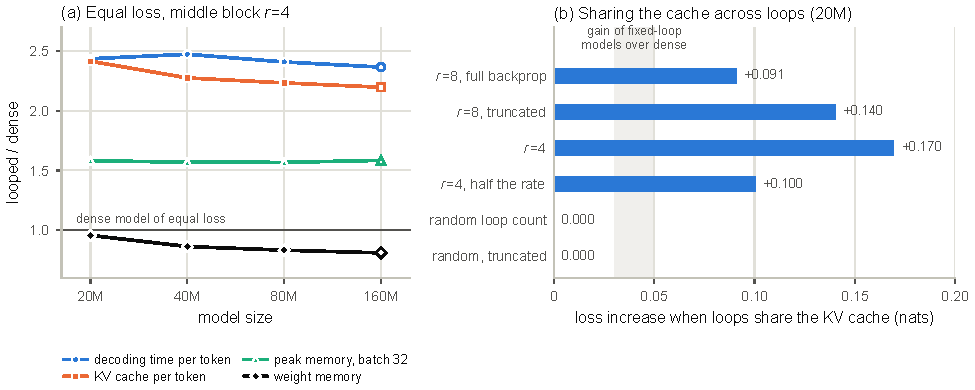
\includegraphics[width=\linewidth]{fig8_deployment}
  \caption{Deployment cost. \textbf{(a)}~A middle block looped 4 times against the dense model of equal loss at $40N$:
  ratios of decoding time per token (batch 1), KV cache per token, peak memory at batch 32 (1k context) and weight
  memory (open markers: 160M lies beyond the largest dense model). \textbf{(b)}~Sharing the KV cache across loops after
  training (20M, one cache slot per unique layer, written at a position's last loop): the loss increase on the main
  set; the shaded band is the fixed-loop models' gain over the dense model of the same size.}
  \label{fig:cost}
\end{figure}

\section{The synthetic task}
\label{app:synthetic}

\paragraph{Data and training.} Tokens are the values 0--96 and a few markers (start, separator, lookup, answer and
padding); a problem is a start value followed by $d$ steps of the form \texttt{LUT k ;}, with the table index $k$
written as one of the value tokens 0--31, and the answer marker. Problems are drawn online. During
the first half of training the largest step count grows linearly from 1 to 8; the second half draws uniformly from
1--8. Models have width 256 and attention heads of dimension 64, and the looped models use the input injection and
residual scaling of the language models. Training uses AdamW ($\beta = (0.9, 0.95)$, weight decay 0.1, gradient clipping
1.0), 400 warm-up steps and a cosine decay to a tenth of the peak rate, 512 problems per step, 32{,}000 steps. The two
deepest conditions of S5 and S9 accumulated gradients over two half-batches to fit in memory (the same loss and update).
Probes are linear maps from the state after each loop (or layer) to the 97 values, trained on 4000 problems with 8 steps
and tested on 1000, at the table-index, separator and next-operation positions of each step, keeping the best.

\paragraph{Learning rates.} The sweep (seed 1; $2.5\times10^{-4}$, $5\times10^{-4}$ and $10^{-3}$, extended at an
edge) chose by mean in-range accuracy at the condition's own loop count: dense 8 and 20 layers $10^{-3}$, dense 36 layers
$5\times10^{-4}$, looped $r = 2$ and $r = 8$ $2.5\times10^{-4}$, looped $r = 4$, random loop count, loops = steps, the S9
model and the chain-of-thought models $1.25\times10^{-4}$, the pause model $5\times10^{-4}$. These are the rates of the
embedding and output layers; the hidden layers use $(L/12)^{-1/2}$ times them, with $L$ the number of unique layers (1.22, 0.77 and 0.58 for 8, 20 and 36), so the hidden layers of the 36-layer
dense model train at about the rate of the 2- and 8-loop models. The criterion saturates at low rates (the loops = steps model scored 0.9999 at three rates and the chain-of-thought models
1.000 at all four), such ties went to the lowest rate by implementation, a rule the protocol had not specified, and the
4-loop, random-loop and S9 models were best at the lowest rate tried. Extrapolation is sensitive to this choice: in the
sweep, the accuracy of the loops = steps model on 9 to 14 steps fell from 1.00 to 0.91 at $2.5\times10^{-4}$ but to 0.05
at $1.25\times10^{-4}$.

\paragraph{Probes.} The \emph{frontier} is the first loop at which each value becomes decodable (probe accuracy
$\geq 0.5$), and \emph{persistence} is the lowest probe accuracy a value reaches in the loops after that, averaged
over the values (Figure~\ref{fig:probes}). In 5 of the 10 seeds of the 20- and 36-layer dense models no
intermediate value after the first appears at the step positions: four show only $x_1$ (probe accuracy 0.50--0.74)
and, at the last layer, the answer, and one shows nothing. Measured by the share of values that first become
decodable at their own loop, a reading of the design's diagonal share fixed after the results, the loops = steps and
8-loop models are diagonal (0.95 and 0.975) and the others are not (0.125); read as the share decoded most accurately
at their own loop, they are 0.625 and 0.425.


\paragraph{S2.} Its plan identified the conditions with 4 and 8 loops, the random loop count and loops = steps as
extrapolating and left out $r = 2$ on the strength of a number corrected later (Appendix~\ref{app:deviations}). Probes of
all sweep checkpoints \lbl{(exploratory)} show the step-by-step frontier at rates up to $5\times10^{-4}$ and not above, for 4 and 8 loops and the random loop
count alike. At $10^{-3}$ the runs that did not learn the training range reached 0.49--0.98 in range; at $5\times10^{-4}$
the runs that learned it extended about as far as the formal runs (8 loops: 2.7
steps beyond the range against 3.2; loops = steps: 4.0 against 4.8), except the random loop count (2 against 4.2).

\paragraph{Where the chain of thought breaks.} As soon as the prompt holds more than 8 tables, the first wrong token
of the 8-layer chain-of-thought model is one of the first three written ones in 97--98\% of the problems, and even
when the correct earlier tokens are given, the tokens after the first two are mostly wrong (accuracy 0.04--0.10)
\lbl{(exploratory)}.

\paragraph{Stopping rules.} Figure~\ref{fig:stopping} shows the confidence rule against the chain length. The plan's selection rule, the highest accuracy over 9--16 steps
on the selection set among rules that keep the in-range accuracy within 0.01 of the training loop count's, also
admitted votes over loop counts and picked a vote for three of the five conditions; without votes it picks the 0.5\%
state rule for $r = 4$, the confidence rule at 0.99 for $r = 8$ and the random loop count, and at 0.9 for $r = 2$; for S9
it picks the 0.5\% state rule with or without votes. Where it picked a vote, the vote runs all 32 loops and comes within
0.013 of the best fixed count without beating it.

\begin{figure}[h]
  \centering
  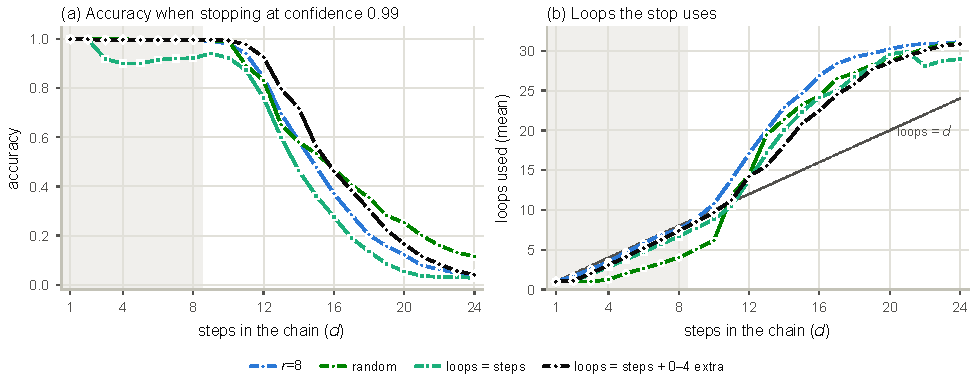
\includegraphics[width=\linewidth]{fig7_stopping}
  \caption{Stopping when the model's top probability reaches 0.99 (reporting set, mean over five seeds).
  \textbf{(a)}~Accuracy. \textbf{(b)}~Loops used: the stop runs few loops on short chains and many on long ones. The
  model trained with loops = steps loses part of the training range; trained with a few random extra loops, it keeps the
  training range and stops best of the four beyond it, up to 15 steps.}
  \label{fig:stopping}
\end{figure}

\paragraph{The pre-specified predictions.} Table~\ref{tab:p1p5} lists the verdicts.

\begin{table}[h]
  \centering
  \caption{The predictions of the frozen synthetic design and their verdicts.}
  \label{tab:p1p5}
  \small
  \begin{tabular}{p{0.38\linewidth}p{0.55\linewidth}}
    \toprule
    Prediction & Verdict \\
    \midrule
    P1: the largest solvable length rises from dense 8 layers to $r = 2, 4, 8$; $r = 8$ reaches 16 & Holds in direction (4.2,
    6.4, 8.0, 9.0); $r = 8$ does not reach 16. \\
    P2: dense models of equal depth are not worse, and the gap is at most a quarter of the dense-8 to looped gap & Not
    supported as stated: they solve 1--1.6 fewer steps, within the tolerance for $r = 8$, not for $r = 4$. \\
    P3a: fixed-loop models lose accuracy sharply at other loop counts & Half right: with fewer loops accuracy drops (the
    8-loop model keeps 0.67 in range at 4 loops); with more loops the 4- and 8-loop models do not, in the direction that favours looping (with 16
    loops the 8-loop model keeps 0.997 in range and solves 11.0 steps instead of 9). \\
    P3b: the random-loop model does not improve with more loops beyond 8 steps & Fails: it gains on long chains (0.08 to
    0.49 at 16 steps). \\
    P3c: the loops = steps model with $d$ loops beats 8 loops beyond 8 steps, to at least 16 & Holds (by 0.34--0.95 at
    every length from 10 to 16; the start at 10 steps and the 0.1 margin were fixed after the results, and at 9 steps the
    gain is 0.03). \\
    P4: only the loops = steps model's probe table is diagonal & Half right: diagonal shares 0.95 (loops = steps) and 0.975
    (8 loops), 0.125 for the others, by a definition fixed after the results; read as the loop at which a value is decoded
    most accurately, they are 0.625 and 0.425, and P4 would hold. \\
    P5: the gaps are much larger than on text & Holds. \\
    \bottomrule
  \end{tabular}
\end{table}

\paragraph{Supplementary predictions.} S2: a high learning rate mainly prevents learning (Section~\ref{sec:lrsynthetic}).
S5 held one of three: the 8-layer chain-of-thought model was predicted to extend at least as far as the looped models
($\geq 0.7$ at 12 steps) and reached 0.014; pause tokens were predicted to add less than 0.1 and added nothing; the
36-layer chain-of-thought model was predicted to reach 0.8 at 12 steps and reached 0.017. S8 held two of five
(Table~\ref{tab:s8}): the prediction rule stayed within 1.5 times the own loop count in range, and votes did not beat the
best fixed count; the prediction rule neither beat the state rule nor recovered 85\% of the gain, and the confidence rule
brought the loops = steps model to 0.76, above the predicted ceiling of 0.2. S9 held three of four; the one that failed is the frozen state rule's stop (0.52 at 12 steps
against a predicted 0.6).

\begin{table}[h]
  \centering
  \caption{S8, all rule families on the reporting set: accuracy at 12 / 16 steps (mean loops used at 12 steps). The
  rule the plan's selection criterion picks is in the last column.}
  \label{tab:s8}
  \footnotesize
  \setlength{\tabcolsep}{3.5pt}
  \begin{tabular}{lcccccc}
    \toprule
    Model & Own loops & Best fixed & State $<0.02$ & Prediction unchanged & Confidence $\geq 0.99$ & Selected \\
    \midrule
    $r=2$ & 0.05 / 0.04 & 0.62 / 0.33 & 0.45 / 0.20 (29) & 0.56 / 0.21 (6.3) & 0.70 / 0.30 (8.3) & confidence $\geq 0.9$ \\
    $r=4$ & 0.04 / 0.02 & 0.83 / 0.29 & 0.65 / 0.21 (11) & 0.48 / 0.09 (6.7) & 0.81 / 0.26 (9.2) & vote, loops 8--32 \\
    $r=8$ & 0.04 / 0.03 & 0.86 / 0.37 & 0.71 / 0.23 (17) & 0.09 / 0.04 (5.5) & 0.84 / 0.37 (17) & vote, loops 8--32 \\
    Random & 0.77 / 0.08 & 0.83 / 0.48 & 0.73 / 0.37 (11) & 0.28 / 0.11 (5.0) & 0.83 / 0.47 (14) & vote, loops 8--32 \\
    Loops = steps & 0.96 / 0.36 & 0.96 / 0.36 & 0.03 / 0.03 (25) & 0.21 / 0.06 (8.8) & 0.76 / 0.28 (14) & none eligible \\
    \bottomrule
  \end{tabular}
\end{table}

\paragraph{Pointer chasing.} The design's second task, following a random function given in the prompt for $k$ hops,
was not learned by any of the four conditions tried on it under the recipe calibrated on the chain task: the 36-layer
dense and 8-loop models, two seeds each, reached 0.10--0.24 accuracy when trained to the end, and the random-loop and
loops = steps models were stopped at 0.13 training accuracy; single-hop retrieval was not learned in that format either.
It was dropped before any comparison on it.

\section{Deviations and corrections}
\label{app:deviations}

Every item is dated in the deviation log in the repository. Among the corrections, the reviews found a verdict judged
with a quantity the frozen design did not specify, a misread synthetic prediction (P3a) and two readings fixed after the
results that the paper had not marked (P3c, P4).
\begin{itemize}
  \item Before any data, the pre-registered training data (sample-100BT) were replaced by sample-10BT, which removed the
  $80N$ point of the 160M dense model, and the pre-registered data point, the mean of a cooldown's last three
  evaluations, by its final evaluation (Appendix~\ref{app:prereg}).
  \item Two power failures of the training machine cut CPU speed for a time; runs resumed from checkpoints and no result
  was affected.
  \item The synthetic task changed twice before its formal runs, both times for learnability and before any comparison
  between conditions: a uniform mixture of 1--8-step problems was not learned (a curriculum was added), and modular
  arithmetic chains were learned too slowly (fixed random lookup tables replaced them). Training was lengthened to
  32{,}000 steps for every condition, three seeds were added to the first two (declared before their results), and the
  probe was widened from one to three positions per step after a diagnostic showed values stored at other positions.
  \item The learning-rate criterion of the synthetic task saturated, and ties went to the lowest rate by implementation
  (Appendix~\ref{app:synthetic}).
  \item Three reviews corrected the results and the paper. The first (2026-10-14) found five errors: a verdict on the
  random-loop model judged by the longest solvable chain instead of the accuracy difference the design specified, a
  double-counted KV cache in the S3 memory figures, an information criterion for H3 that was only a Huber-loss proxy (no
  longer cited), an extrapolation test of H3 that had kept 160M in its training set, and a design statement that problems
  never repeat, false for short ones. The second (2026-10-15) corrected about 35 numbers and statements, among them the
  verdicts on P3c and P4, the equal-compute claim (now limited to the measured range), a statement that the loops = steps
  model overwrites its values (it keeps them within its $d$ loops), a 12-step comparison with dense models that had mixed
  in extra loops and a best over loop counts that had left out some counts; it also reported an evaluation the frozen
  design specified, the state-rule stop of the loops = steps model, which had been computed but not reported. The third
  (2026-10-27), of the paper itself, corrected the S8 count (two of five predictions held), two rounding errors, the
  claim that confidence is the best stopping rule in every condition, the count of voided results, the P3a verdict and
  the chain of thought's breaking point, added the pre-data changes to the pre-registration and the outcomes of the S4,
  S6 and S7 predictions, and marked the readings fixed after the results (P3c, P4). Every item is dated in the log.
  \item Two synthetic conditions of S5 and S9 ran out of GPU memory at the planned batch, having been tested only on a CPU
  before their plan was frozen; they were rerun with two accumulated half-batches.
  \item S10 (plan frozen 2026-10-27): its analysis script flagged that the learning-rate rule applied at 40M and $10N$
  but did not compute the readings at the best rate; a script written after the results computes them
  (Appendix~\ref{app:s10}). The script's intervals for the paired gap are not resampled, so the per-seed gaps are
  reported instead. The checkpoint size stated earlier (485 GB, measured on 2026-10-15) was not updated as S4--S10
  added checkpoints; it is about 560 GB.
  \item One unexplained anomaly: at 160M one looped seed is 0.2--0.6 nats worse than the other on the
  out-of-distribution sets at $40N$, while their main-set losses are identical.
\end{itemize}
